\documentclass[a4paper,12pt]{article}
\usepackage{outline}
\usepackage{pmgraph}
\usepackage[normalem]{ulem}
\usepackage{comment} % enables the use of multi-line comments (\ifx \fi)
\usepackage{lipsum} %This package just generates Lorem Ipsum filler text.
\usepackage{fullpage} % changes the margin
\usepackage{listings}
\usepackage{color}
\usepackage{mdframed}
\usepackage{listings}
\usepackage{graphicx}
\graphicspath{ {../ScreenShots/} }
\renewcommand{\lstlistingname}{Code Block}% Listing -> Algorithm
\renewcommand{\lstlistlistingname}{List of \lstlistingname s}% List of Listings -> List of Algorithms

\linespread{1.5}
%--------------------Indention
\setlength{\parindent}{15pt}
\lstset{frame=shadowbox, rulesepcolor=\color{white}}
\mdfsetup{frametitlealignment=\center}
\lstset{
  numbers=left,
  stepnumber=1,
  firstnumber=1,
  numberfirstline=true
}

\begin{document}
\section*{Objective}

\hspace{15pt}In the last lab, two different methods to create digital circuits in Verilog was introduced. One was
structural method and the other was dataflow modeling. In this lab, a $3^{rd}$ method will be used, behavioral modeling.

This lab consisted of three separate experiments. For \textbf{Experiment 1}, the multiplexers created last lab will
be converted into behavioral Verilog. In \textbf{Experiment 2}, students will describe, using behavioral Verilog, binary encoders and decoders. Finally, \textbf{Experiment 3} will introduce logic synthesis, as well as translating HDL code into implementable digital logic. The code written in Experiment 2 will be synthesized and programmed onto a Spartan 3E in order to further verify that the encoder and decoder described is in fact correct.

\section*{Design}

\textbf{Experiment 1}

  \vspace{15pt}In the first experiment, the student was able to practice their newly formed
  knowledge of behavioral Verilog by converting preiovosly created structaul code
  into behavioral. There were three separate conventions, one for a \textit{1-
  Bit 2:1 MUX}, another for a \textit{4-Bit 2:1 MUX}, and finally \textit{4-
  Bit 4:1 MUX.} The following is the code wirtten for each convertion.

  \lstinputlisting[language=Verilog,,caption=1-Bit 2:1 MUX Behavioral ]{../Code/two_one_mux_behavioral.v}

  \lstinputlisting[language=Verilog,,caption=4-Bit 2:1 MUX Behavioral ]{../Code/four_bit_mux_behavioral.v}

  \lstinputlisting[language=Verilog,,caption=4-Bit 4:1 MUX Behavioral ]{../Code/mux_4bit_4tol.v}

  \hspace{-15pt}\textbf{Experiment 2}

  \vspace{15pt}In the second experiment, the student was able to move into creating
  new behavioral code for the first time. A 2:4 decoder, 4:2 encoder, and a priority
  encoder were all implemented. All of which had not been mentioned in lecture.

  \lstinputlisting[language=Verilog,,caption=2:4 Decoder ]{../Code/two_four_decoder.v}

  \lstinputlisting[language=Verilog,,caption=4:2 Encoder ]{../Code/four_two_encoder.v}

  \lstinputlisting[language=Verilog,,caption=Priority Encoder ]{../Code/priority_encoder.v}

  \hspace{-15pt}\textbf{Experiment 3}

  \vspace{15pt}In the final experiment, no new code was written but the code
  written in experiment 2 was implemented onto the Spartan 3E board in lab.
  The components on the board allows the student to confirm that the code created
  actually functions. The buttons and LEDs on the board were used for input and
  output.

  \section*{Results}

  \textbf{Experiment 1}

  \vspace{15pt}In the first experiment, the three MUX designs were tested against
  the appropriate test benches. The following are the results of these tests.
  All the tests passed in all three cases.

  \begin{figure}[h]
    \begin{center}
      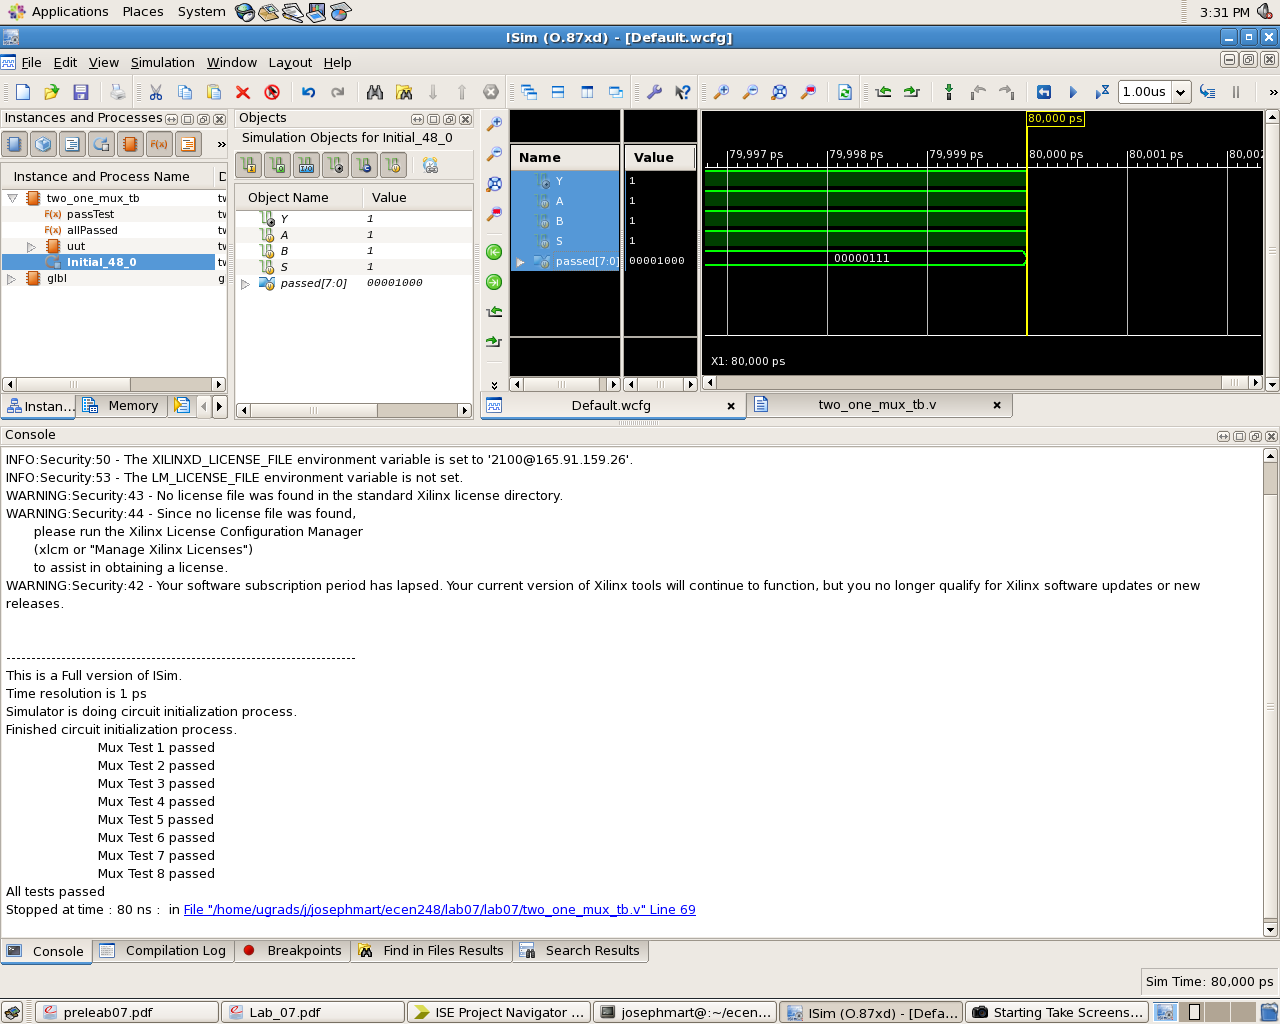
\includegraphics[scale=0.18]{1_1_1.png}
      \caption{\textit{1-Bit 2:1 Mux Behavioral Tests}}
    \end{center}
  \end{figure}

  \newpage

  \begin{figure}[h]
    \begin{center}
      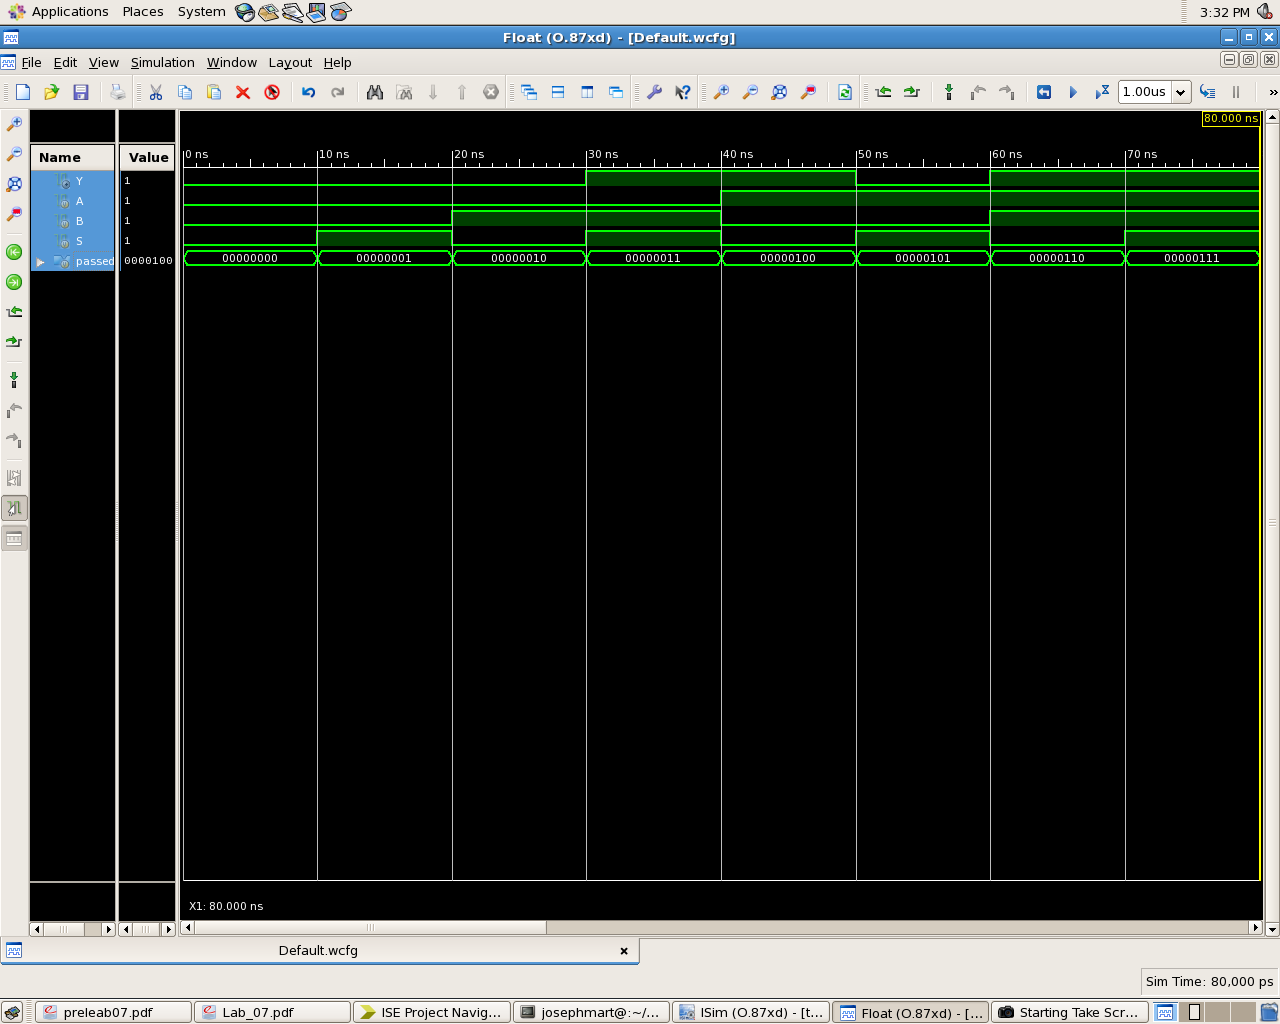
\includegraphics[scale=0.18]{1_1_2.png}
      \caption{\textit{1-Bit 2:1 Mux Behavioral Graph}}
    \end{center}
  \end{figure}

  \begin{figure}[h]
    \begin{center}
      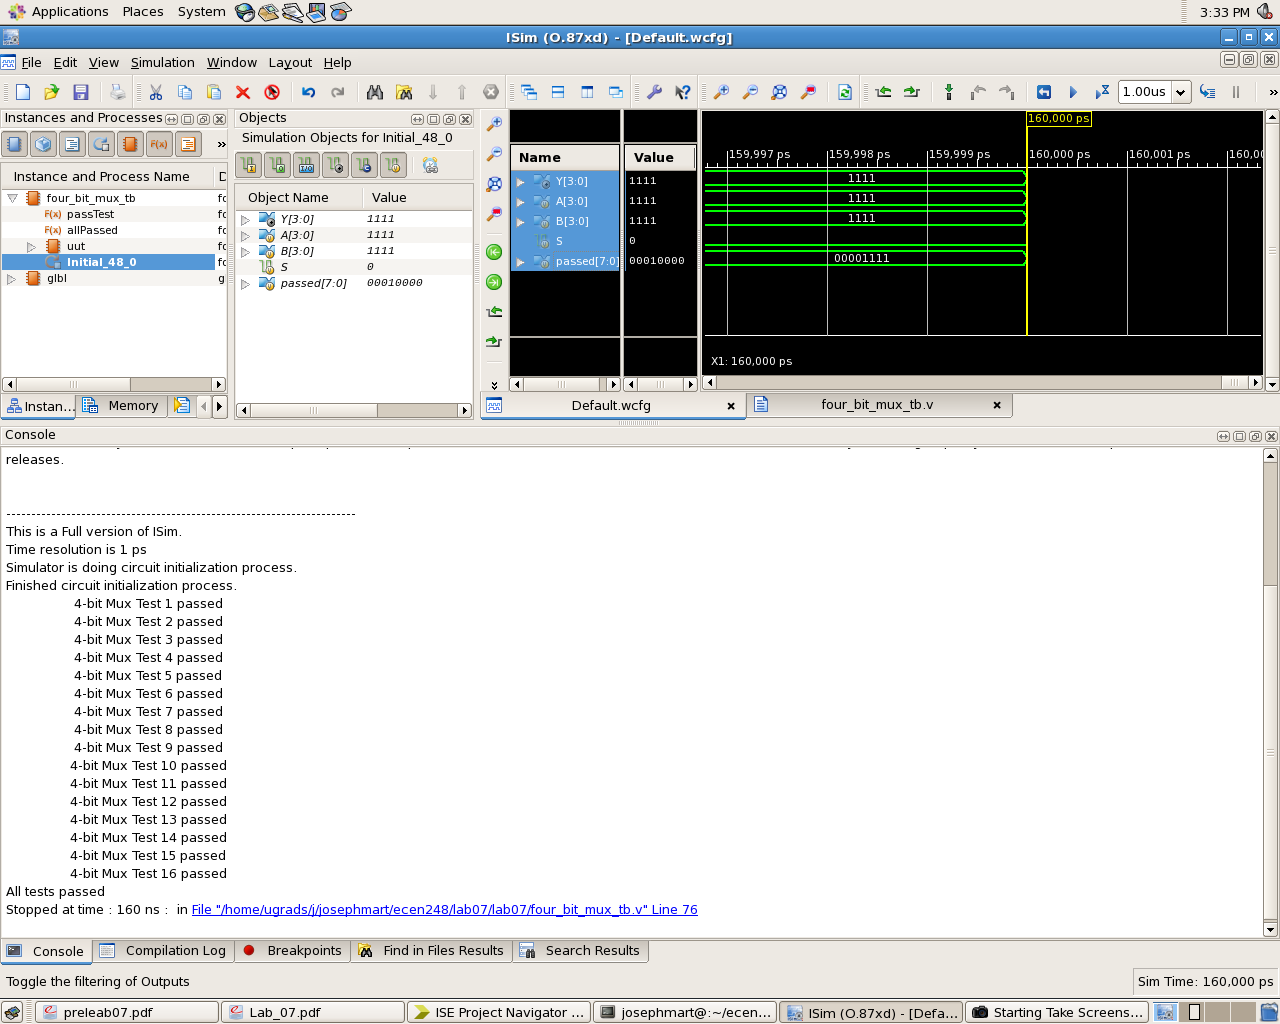
\includegraphics[scale=0.18]{1_2_1.png}
      \caption{\textit{4-Bit 2:1 MUX Behavioral Tests}}
    \end{center}
  \end{figure}

  \newpage

  \begin{figure}[h]
    \begin{center}
      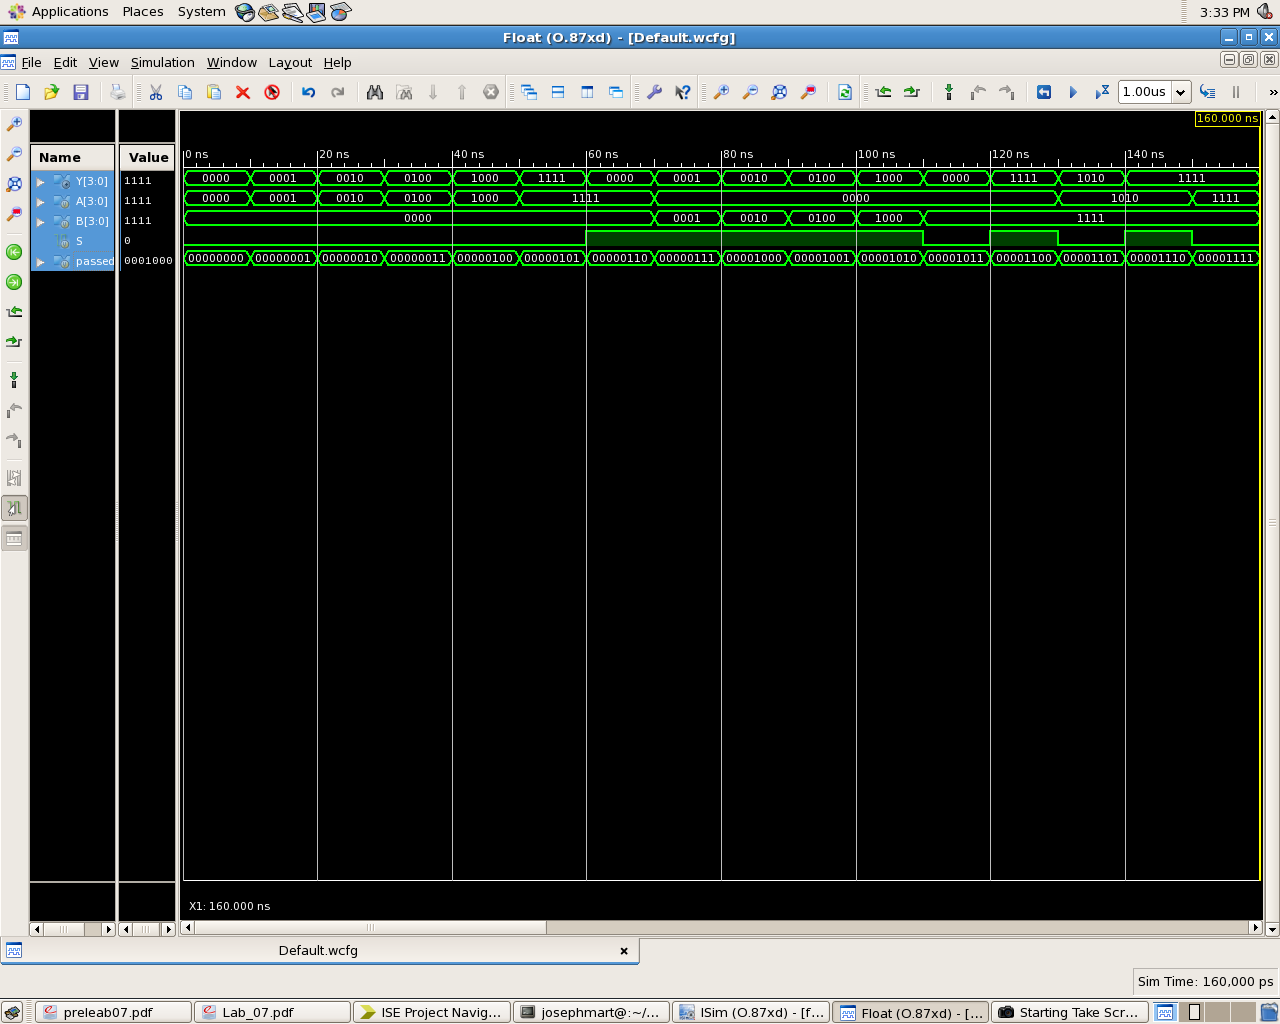
\includegraphics[scale=0.18]{1_2_2.png}
      \caption{\textit{4-Bit 2:1 MUX Behavioral Graph}}
    \end{center}
  \end{figure}

  \begin{figure}[h]
    \begin{center}
      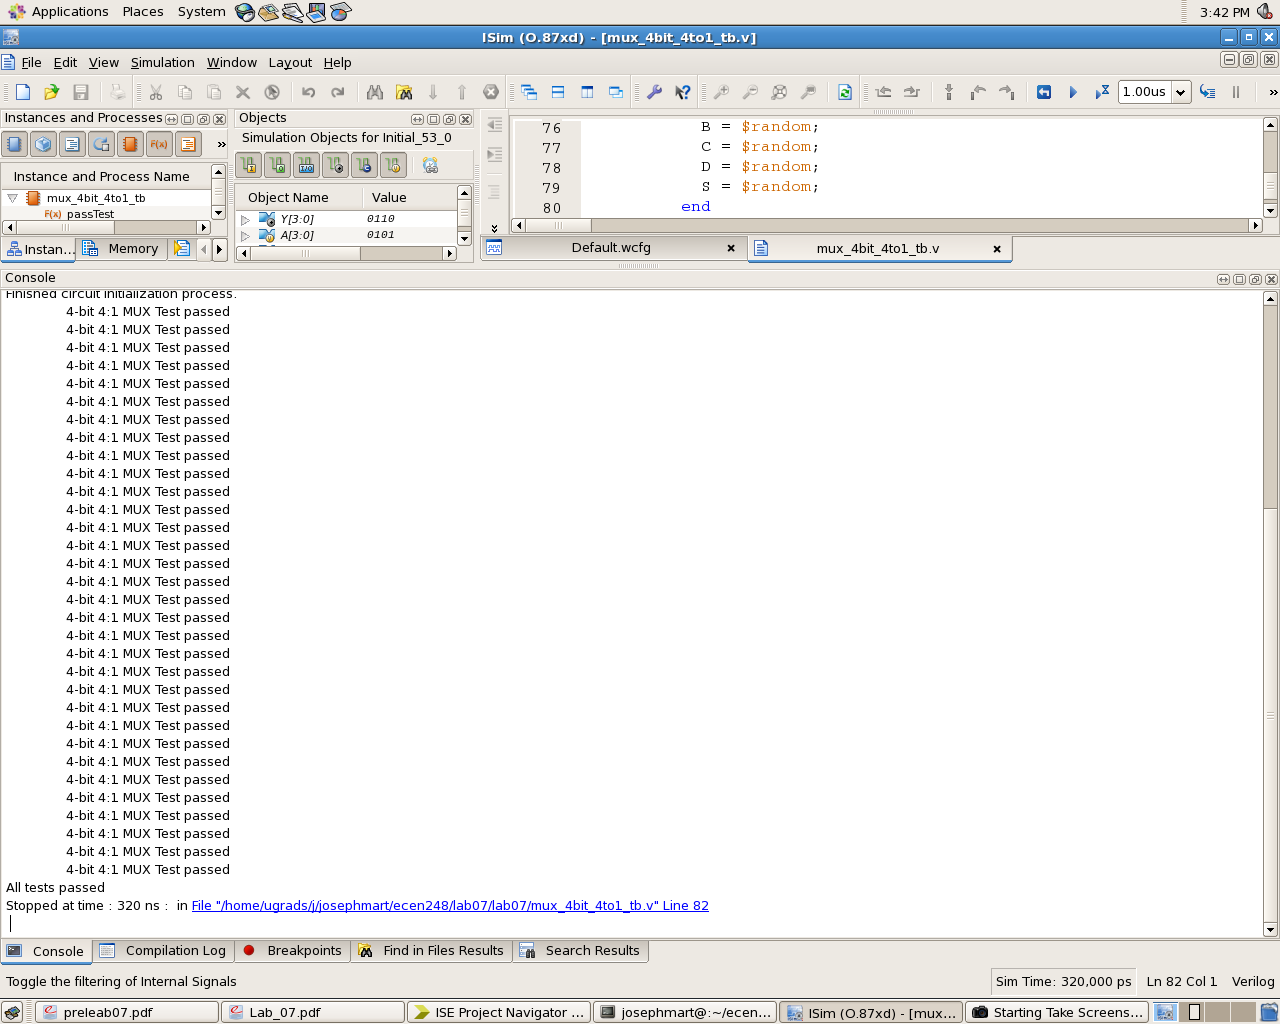
\includegraphics[scale=0.18]{1_3_1.png}
      \caption{\textit{4-Bit 4:1 MUX Behavioral Tests}}
    \end{center}
  \end{figure}

  \newpage

  \begin{figure}[h]
    \begin{center}
      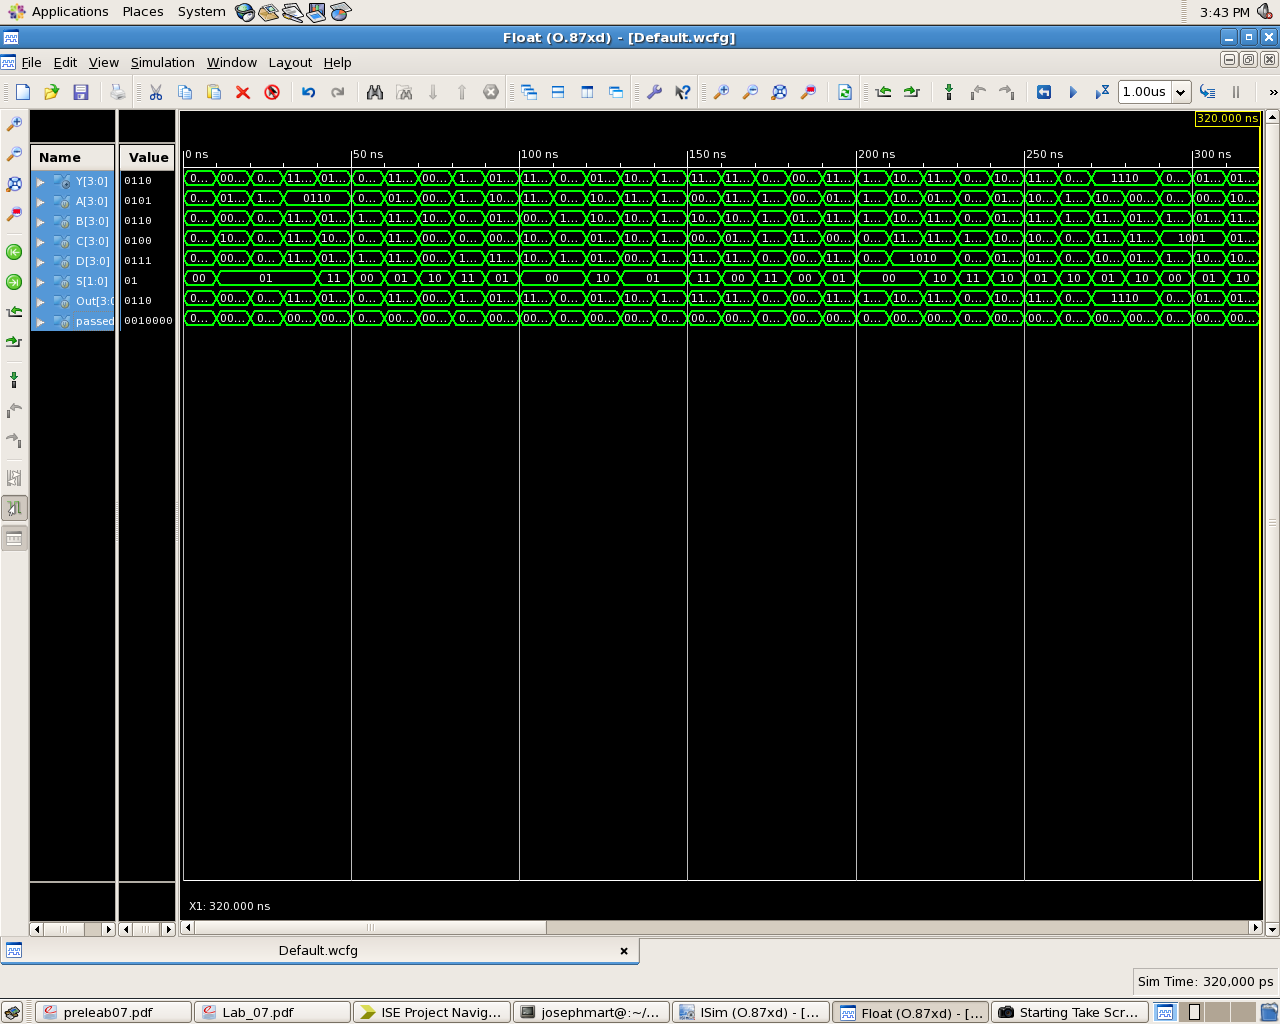
\includegraphics[scale=0.18]{1_3_2.png}
      \caption{\textit{4-Bit 4:1 MUX Behavioral Graph}}
    \end{center}
  \end{figure}

  \hspace{-15pt}\textbf{Experiment 2}

  \vspace{15pt}In the second experiment, the 2:4 decoder, 4:2 encoder, and the
   priority encoder were all tested against the appropriate test benches. The
   following are the results of these tests. All the tests passed in all three cases.

  \begin{figure}[h]
    \begin{center}
      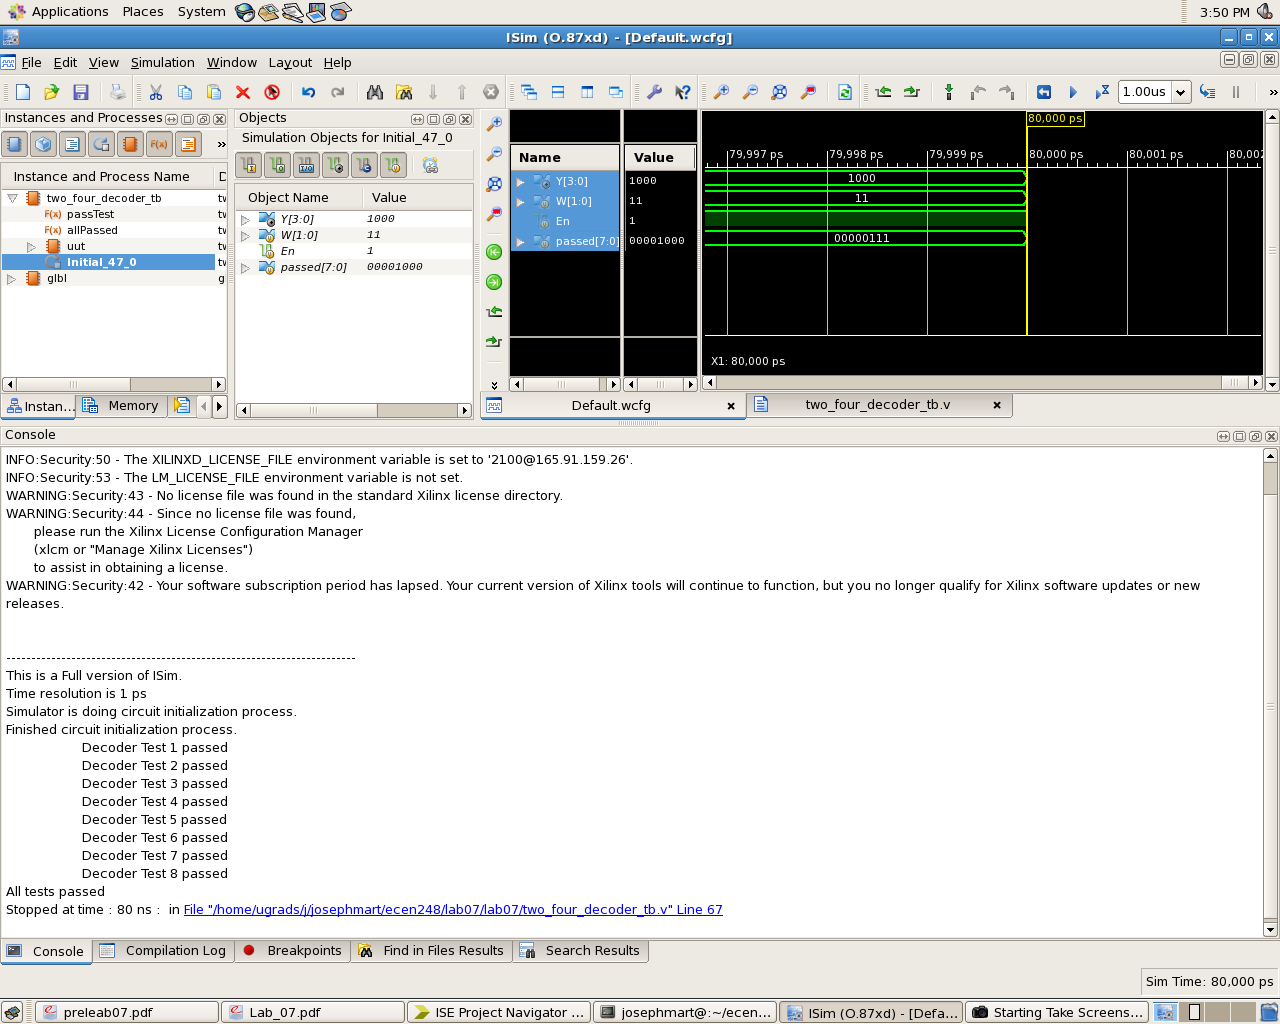
\includegraphics[scale=0.18]{2_1_1.png}
      \caption{\textit{2:4 Decoder Tests}}
    \end{center}
  \end{figure}

  \newpage

  \begin{figure}[h]
    \begin{center}
      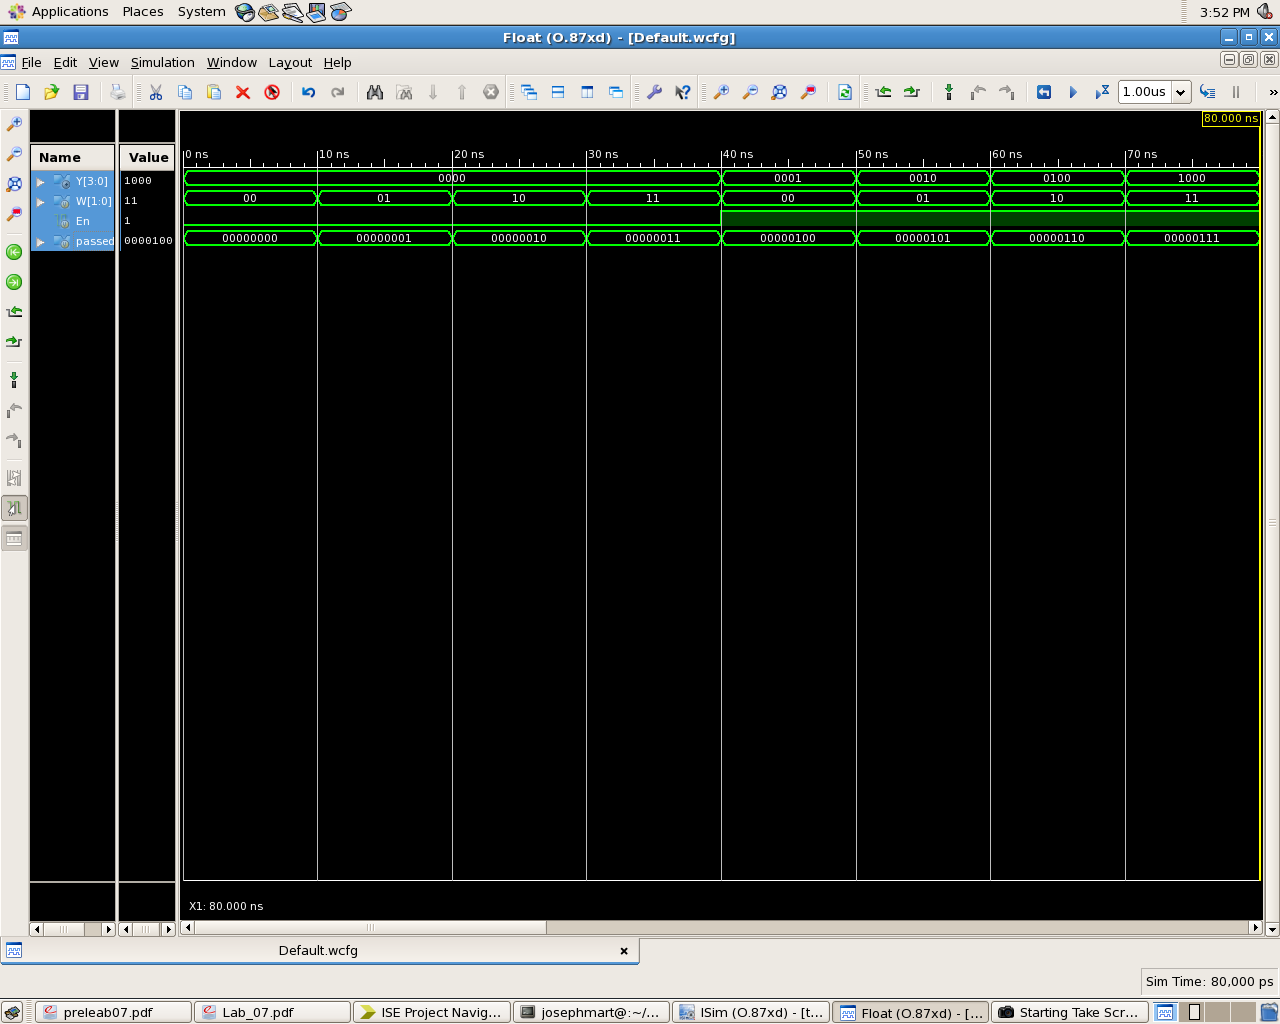
\includegraphics[scale=0.18]{2_1_2.png}
      \caption{\textit{2:4 Decoder Graph}}
    \end{center}
  \end{figure}

  \begin{figure}[h]
    \begin{center}
      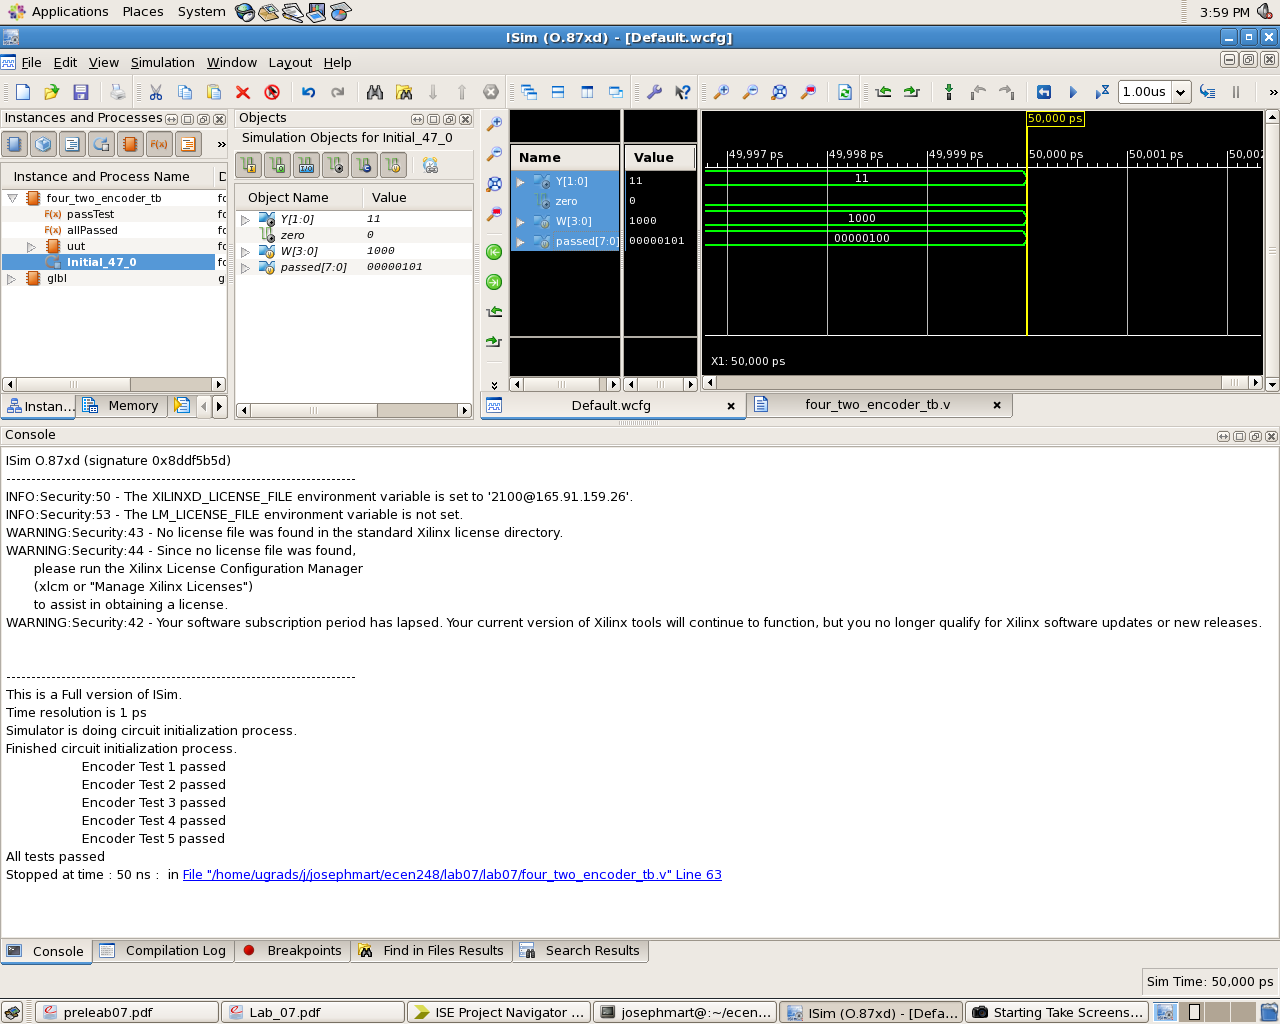
\includegraphics[scale=0.18]{2_2_1.png}
      \caption{\textit{4:2 Encoder Tests}}
    \end{center}
  \end{figure}

  \newpage

  \begin{figure}[h]
    \begin{center}
      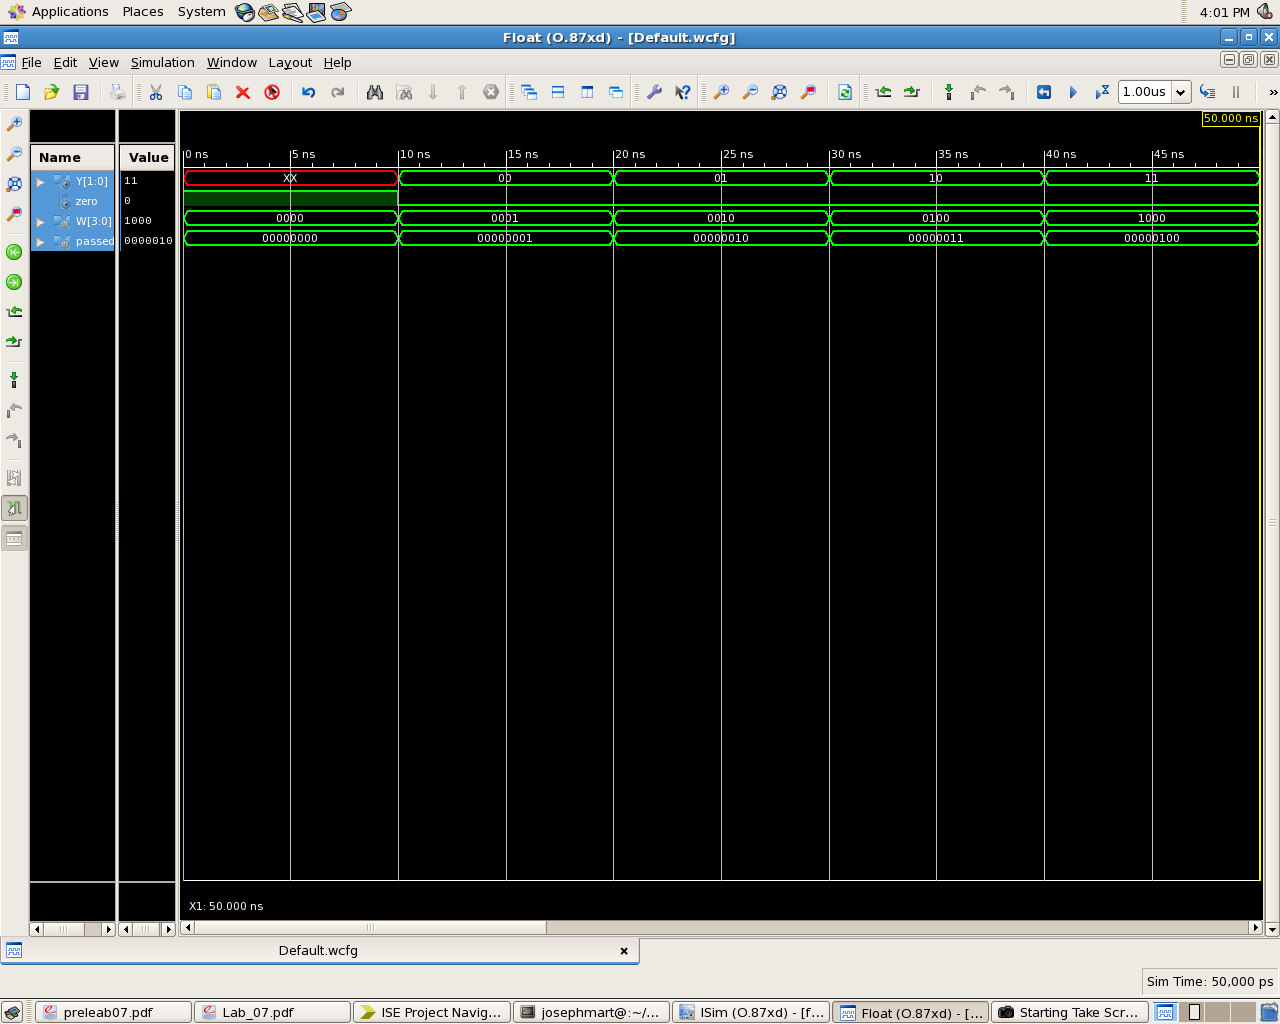
\includegraphics[scale=0.18]{2_2_2.png}
      \caption{\textit{4:2 Encoder Graph}}
    \end{center}
  \end{figure}

  \begin{figure}[h]
    \begin{center}
      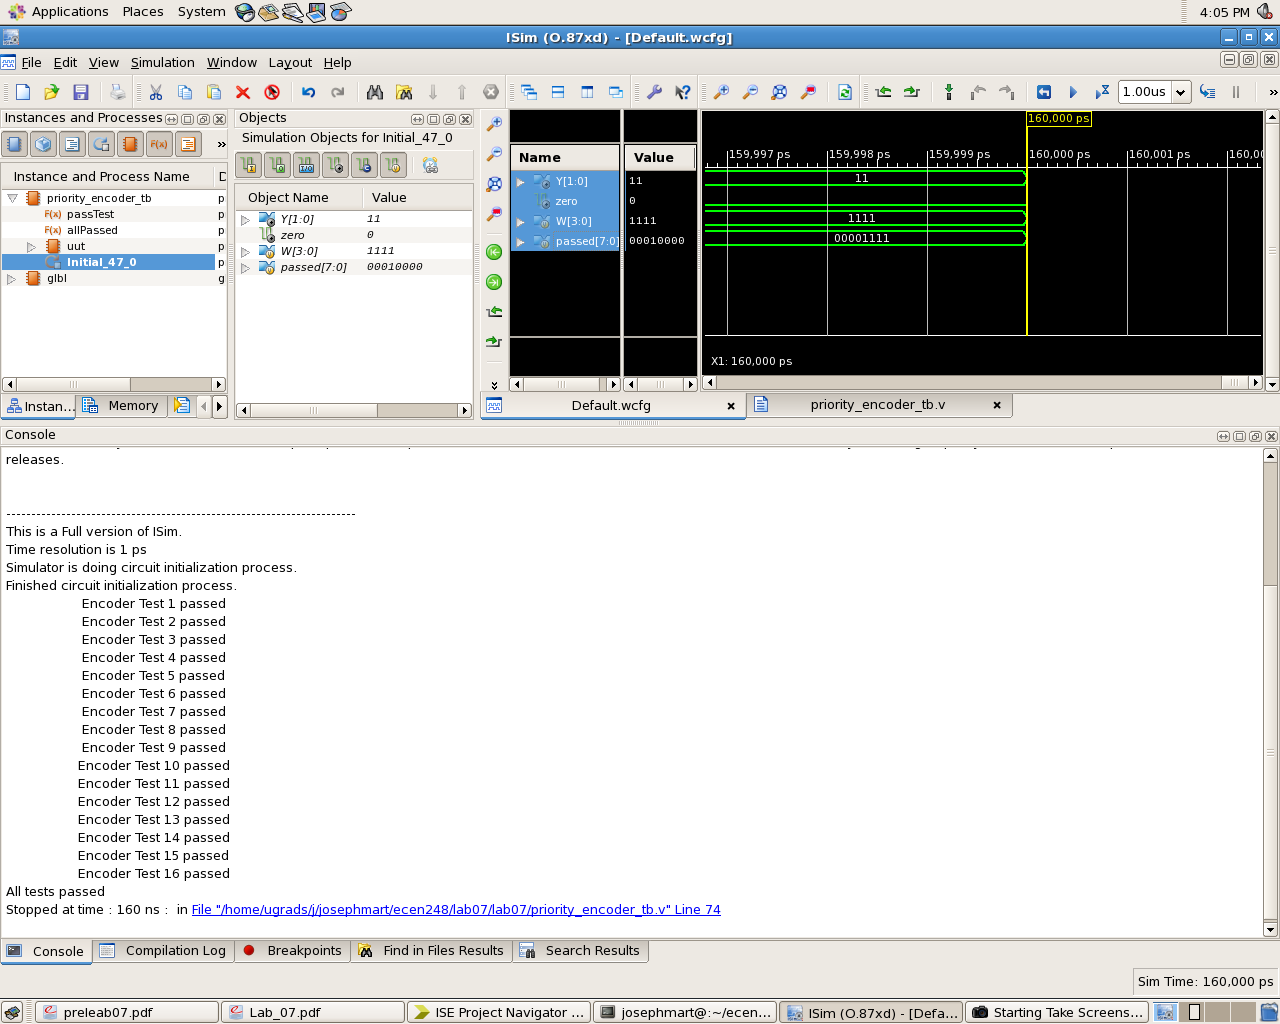
\includegraphics[scale=0.18]{2_3_1.png}
      \caption{\textit{Priority Encoder Tests}}
    \end{center}
  \end{figure}

  \newpage

  \begin{figure}[h]
    \begin{center}
      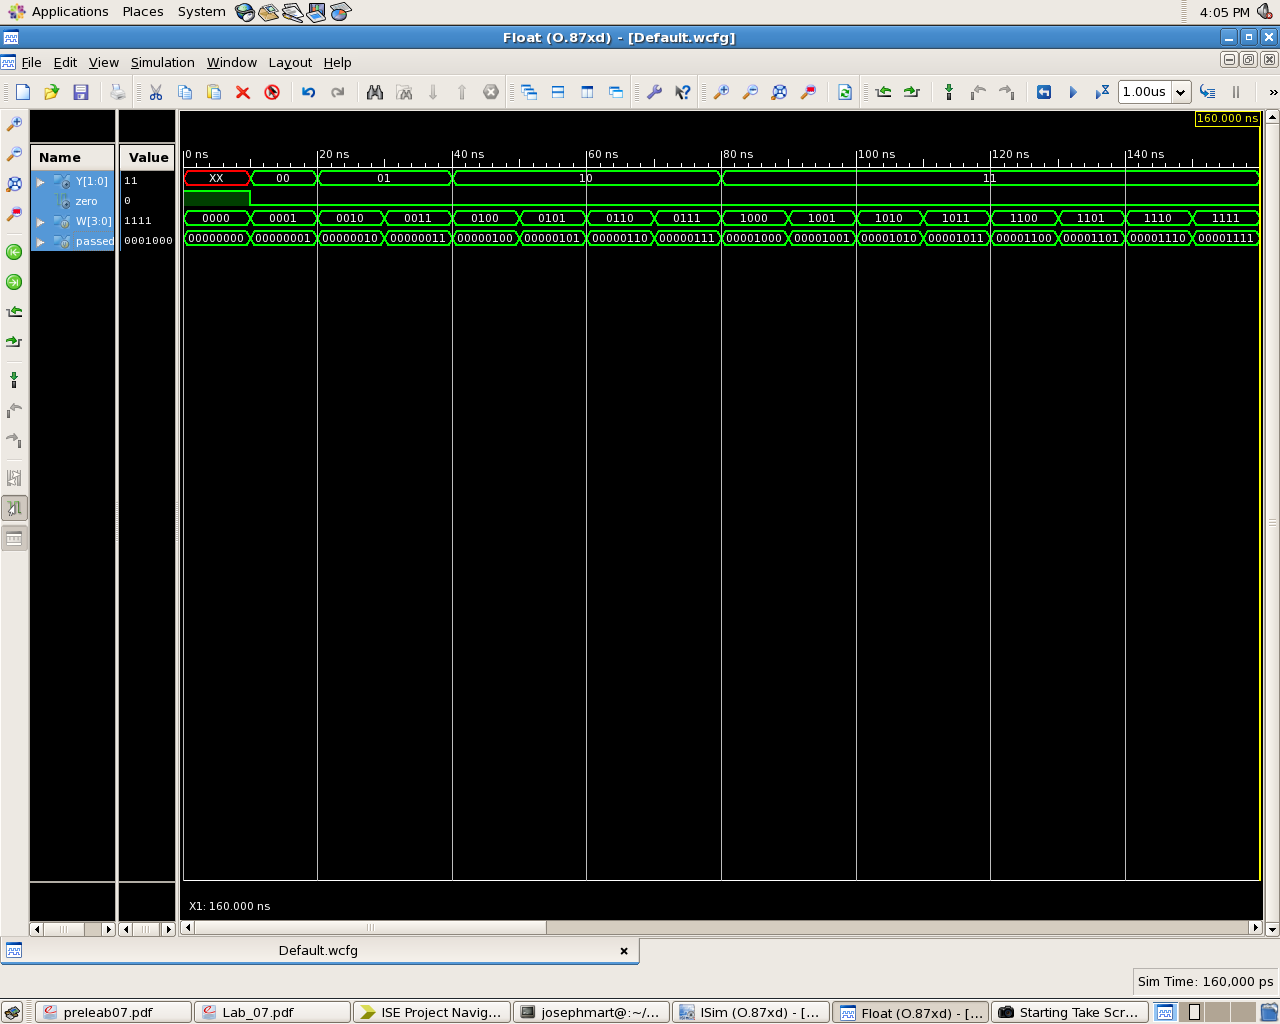
\includegraphics[scale=0.18]{2_3_2.png}
      \caption{\textit{Priority Encoder Graph}}
    \end{center}
  \end{figure}

  \hspace{-15pt}\textbf{Experiment 3}

  \hspace{15pt}In the final part of the lab, the design code was implemented onto
  the board. Buttons on the board were used for input. LEDs were used for output.
  The results were then compared the the proper results similiar to the test
  bench code.

\section*{Conclutions}


\section*{Questions}

\begin{enumerate}
  \item \textbf{Include the source code with comments for all modules you simulated. You do not have to include test bench code. Code without comments will not be accepted!}

  \textit{In Report}

  \item \textbf{Include screen shots of all wave forms captured during simulation in addition to the test bench console output for each test bench simulation.}

  \textit{In Report}

  \item \textbf{Provide a comparison between behavioral Verilog used in this week’s lab and the structural and dataflow Verilog used in last week’s lab. What might be the advantages and disadvantages of each.}

  \textit{Code Block 7} is an example of dataflow Verilog. \textit{Code Block 8} is
  an example of behavioral Verilog. Dataflow is useful when logic gates are
  wanted to be used in the code design. Behavioral Verilog is used when one
  wants to use code similar to other coding languages and implement if statements

  \lstinputlisting[language=Verilog,,caption=Add Sub ]{../Code/add_sub.v}

  \lstinputlisting[language=Verilog,,caption=1-Bit 2:1 MUX Behavioral Code ]{../Code/two_one_mux_behavioral.v}

  \item \textbf{Compare the process of bread-boarding digital circuit to implementing a digital circuit on an FPGA. State some advantages and disadvantages of each. Which process do you prefer?}

  The biggest and most obvious difference is that one is done on a computer (Verilog) and then implemented onto a FPGA the other is physically built (breadboarding). The advantage of Verilog and
  Implementation allows for higher level circuits to be built onto smaller areas. The advantage of a breadboard over FPGA is that it is easier to make changes to components because the size is much larger.

\end{enumerate}

\section*{Student Feedback}

\begin{enumerate}
  \item \textbf{What did you like most about the lab assignment and why? What did you like least aboub it and why?}
  \vspace{10pt}

  I enjoyed implementing my design onto the Spartan board. I did not enjoy having
  to wait for another person to finish their lab so I could use their computer
  because my Spartan board was not functioning.

  \item \textbf{Were there any section of the lab manual that were unclear? If so, what was unclear? Do you have any suggetions for improving the clarity?}
  \vspace{10pt}

  This lab was very straight forward

  \item \textbf{What suggestions do you have to improve the overall lab assignment?}
  \vspace{10pt}

  Better equipment!!

\end{enumerate}

\ifx
\begin{thebibliography}{1}
\bibitem{Verilog} Charles Kime \& Thomas Kaminski  \emph{Logic and Computer Design Fundamentals} \\ \hspace{15pt}\textit{http://www.cs.bilkent.edu.tr/~will/courses/CS223/Verilog/LCDF3_Verilog_Ch_4.pdf}
\end{thebibliography}

\section*{Attachments}
%Make sure to change these
Lab Notes, HelloWorld.ic, FooBar.ic
%\fi %comment me out

\begin{thebibliography}{9}
\bibitem{Verilog} Charles Kime & Thomas Kaminski  \emph{Logic and Computer Design Fundamentals} \textit{http://www.cs.bilkent.edu.tr/~will/courses/CS223/Verilog/LCDF3_Verilog_Ch_4.pdf}
\end{thebibliography}

%How to cite
Put your Problem statement here! Example of a Citation\cite[p.219]{Robotics}. Here's Another Citation\cite{Flueck}
\fi
\end{document}
